\section{Исследование функций и уравнений решения}
1. По теореме Виета $x_1+x_2=4,\ x_1x_2=a.$ Тогда $x_1^2+x_2^2=(x_1+x_2)^2-2x_1x_2=16-2a=16\Rightarrow a=0.$ Дискриминант уравнения в этом случае равен 16, а значит корни существуют и $a=0$ является ответом.\\
2. По теореме Виета $x_1+x_2=2,\ x_1x_2=a.$ Тогда $(x_1-x_2)^2=(x_1+x_2)^2-4x_1x_2=4-4a=16\Rightarrow a=-3.$ Дискриминант уравнения в этом случае равен 16, а значит корни существуют и $a=-3$ является ответом.\\
3. Для нахождения области определения данной функции необходимо решить неравенство\\ $\cfrac{|x-3|(x+4)(x^2+9x+20)}{x^2-x-6}\geqslant0\Leftrightarrow
\cfrac{|x-3|(x+4)^2(x+5)}{(x-3)(x+2)}\geqslant0.$ Применив метод интервалов, найдём ответ:
\begin{figure}[ht!]
\center{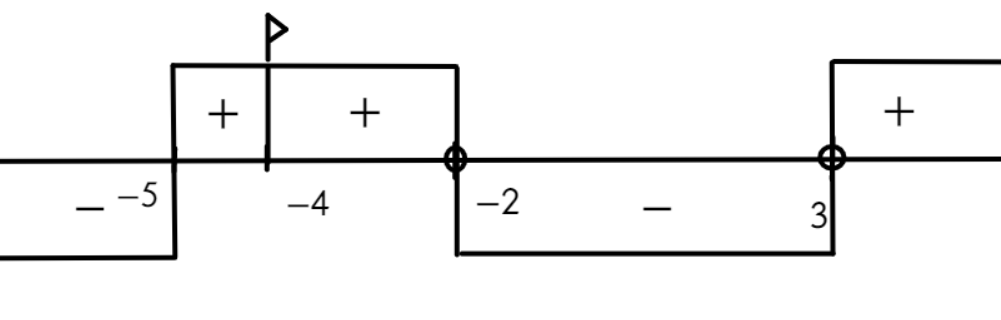
\includegraphics[scale=0.35]{isl3.png}}
\end{figure}
$x\in[-5;-2)\cup(3;+\infty).$\\
4. Для нахождения области определения данной функции необходимо решить неравенство\\ $\cfrac{|x-1|(x+3)(x^2+8x+15)}{x^2+x-2}\geqslant0\Leftrightarrow
\cfrac{|x-1|(x+3)^2(x+5)}{(x-1)(x+2)}\geqslant0.$ Применив метод интервалов, найдём ответ:
\begin{figure}[ht!]
\center{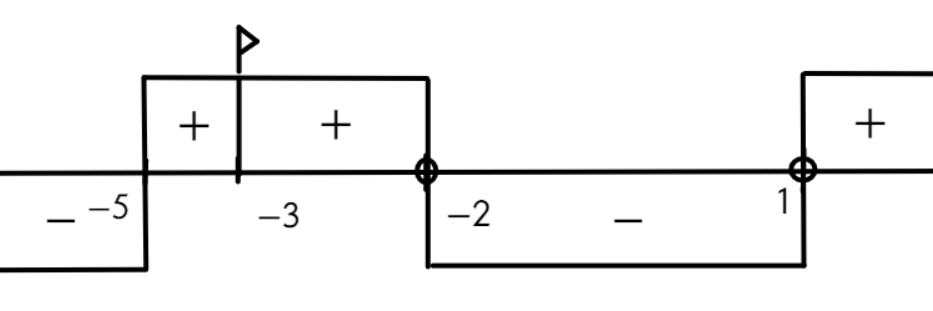
\includegraphics[scale=0.35]{isl4.png}}
\end{figure}
$x\in[-5;-2)\cup(1;+\infty).$\\
5. Пусть $f(x)=ax^2+bx+c.$ Тогда $c\cdot(a+b+c)=f(0)\cdot f(1)<0.$ Значит, на концах отрезка $[0;1]$ функция $f(x)$ принимает значения разных знаков, поэтому где-то на интервале $(0;1)$ её значение равно 0. Иметь только один корень эта функция не может, так как тогда все остальные значения были бы одного знака, что невозможно. Значит, квадратный трёхчлен $ax^2+bx+c$ имеет два корня.\\
6. Пусть $f(x)=ax^2+bx+c.$ Тогда $c\cdot(a-b+c)=f(0)\cdot f(-1)<0.$ Значит, на концах отрезка $[-1;0]$ функция $f(x)$ принимает значения разных знаков, поэтому где-то на интервале $(-1;0)$ её значение равно 0. Иметь только один корень эта функция не может, так как тогда все остальные значения были бы одного знака, что невозможно. Значит, квадратный трёхчлен $ax^2+bx+c$ имеет два корня.\\
7. Возможны два случая: $D=0$ или $k-2=0.$ В первом случае $4(k-1)^2-4k(k-2)=0,\ k^2-2k+1-k^2+2k=0,\ 1=0,$ что невозможно. Во втором случае $k=2,$ что и является ответом.\\
8. Возможны два случая: $D=0$ или $k+2=0.$ В первом случае $4(k+1)^2-4k(k+2)=0,\ k^2+2k+1-k^2-2k=0,\ 1=0,$ что невозможно. Во втором случае $k=-2,$ что и является ответом.\\
9. $y=x^2-7x+6=\left(x-\cfrac{7}{2}\right)^2-\cfrac{49}{4}+6=\left(x-\cfrac{7}{2}\right)^2-\cfrac{25}{4}.$ Наименьшее значение функции достигается, когда квадрат равен 0, а наибольшее --- когда квадрат имеет наибольший модуль (в том из концов отрезка, который дальше от вершины). Значит, наименьшее значение равно $-\cfrac{25}{4},$ а наибольшее ---
$\left(8-\cfrac{7}{2}\right)^2-\cfrac{25}{4}$ или $\left(-1-\cfrac{7}{2}\right)^2-\cfrac{25}{4}.$ Оба потенциально наибольших значения равны 14.\newpage\noindent
10. Для нахождения области определения данной функции необходимо решить неравенство\\ $\cfrac{(x-1)^2(2x-x^2+2)}{(x^2+x-6)|x+2|}\geqslant0\Leftrightarrow
\cfrac{(x-1)^2(x-(1-\sqrt{3}))(x-(1+\sqrt{3}))}{(x-2)(x+3)|x+2|}\leqslant0.$ Применив метод интервалов, найдём ответ:
\begin{figure}[ht!]
\center{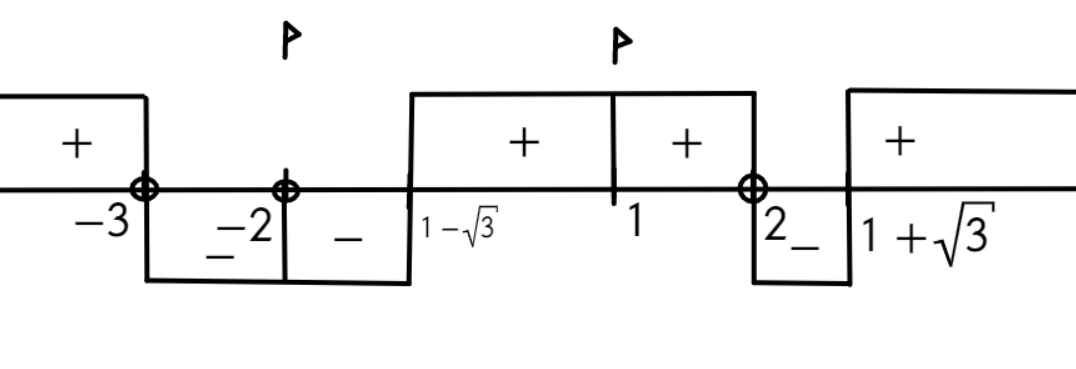
\includegraphics[scale=0.35]{isl10.png}}
\end{figure}
$x\in(-3;-2)\cup(-2;1-\sqrt{3}]\cup\{1\}\cup(2;1+\sqrt{3}].$\\
11. Выразим $x:\ x=4-2y.$ Тогда необходимо найти наименьшее значение выражения $(4-2y)^2-2(4-2y)y+8y^2=16-16y+4y^2-8y+4y^2+8y^2=
16y^2-24y+16=(4y-3)^2+7\geqslant7.$\\
12. Выразим $x:\ x=4+2y.$ Тогда необходимо найти наименьшее значение выражения $(4+2y)^2+2(4+2y)y+8y^2=16+16y+4y^2+8y+4y^2+8y^2=
16y^2+24y+16=(4y+3)^2+7\geqslant7.$\\
13. У этого уравнения есть корни $x=3,\ x=a$ и $x=2a.$ Корней ровно два, а не три, в том случае, если два корня совпадут. Это происходит, если $a=3,\ 2a=3$ или $2a=a.$ Решив эти уравнения, получим ответ: $a\in\{0; 1,5;3\}.$\\
14. У этого уравнения есть корни $x=5,\ x=a$ и $x=2a.$ Корней ровно два, а не три, в том случае, если два корня совпадут. Это происходит, если $a=5,\ 2a=5$ или $2a=a.$ Решив эти уравнения, получим ответ: $a\in\{0; 2,5;5\}.$\\
15. По теореме Виета $x_1+x_2=-10,\ x_1x_2=q.$ Тогда $x_1^2+x_2^2=(x_1+x_2)^2-2x_1x_2=100-2q=2\Rightarrow q=49.$ Дискриминант уравнения в этом случае равен $100-4\cdot49<0,$ а значит таких значений $q$ не существует.\\
16. По теореме Виета $x_1+x_2=10,\ x_1x_2=q.$ Тогда $x_1^2+x_2^2=(x_1+x_2)^2-2x_1x_2=100-2q=2\Rightarrow q=49.$ Дискриминант уравнения в этом случае равен $100-4\cdot49<0,$ а значит таких значений $q$ не существует.\\
17. Сначала разберём случай, когда уравнение не является квадратным: $k-1=0,\ k=1,\ -x+2=0,\ x=2.$ Теперь разберём случай, когда у уравнения один корень:
$(2k-1)^2-4\cdot2\cdot(k-1)=0,\ 4k^2-4k+1-8k+8=0,\ (2k-3)^2=0,\ k=\cfrac{3}{2}.$ В этом случае $x=\cfrac{2k-1}{2(k-1)}=\cfrac{2}{1}=2.$ Во всех остальных случаях $x=\cfrac{2k-1\pm|2k-3|}{2(k-1)}=\left[\begin{array}{l}\cfrac{2k-1+2k-3}{2(k-1)}=2,\\ \cfrac{2k-1-2k+3}{2(k-1)}=\cfrac{1}{k-1}.\end{array}\right.$\\
18. Сначала разберём случай, когда уравнение не является квадратным: $k-1=0,\ k=1,\ x-2=0,\ x=2.$ Теперь разберём случай, когда у уравнения один корень:
$(2k-3)^2+4\cdot2\cdot(k-1)=0,\ 4k^2-12k+9+8k-8=0,\ (2k-1)^2=0,\ k=\cfrac{1}{2}.$ В этом случае $x=\cfrac{2k-3}{2(k-1)}=\cfrac{-2}{-1}=2.$ Во всех остальных случаях $x=\cfrac{2k-3\pm|2k-1|}{2(k-1)}=\left[\begin{array}{l}\cfrac{2k-3+2k-1}{2(k-1)}=2,\\ \cfrac{2k-3-2k+1}{2(k-1)}=\cfrac{1}{1-k}.\end{array}\right.$\\
19. По теореме Виета $x_1+x_2=\cfrac{3}{2},\ x_1x_2=-\cfrac{11}{2}.$ Тогда $\cfrac{x_1}{x_2}+\cfrac{x_2}{x_1}=\cfrac{x_1^2+x_2^2}{x_1x_2}=
\cfrac{(x_1+x_2)^2-2x_1x_2}{x_1x_2}=\cfrac{\cfrac{9}{4}+2\cdot\cfrac{11}{2}}{-\cfrac{11}{2}}=-\cfrac{53}{22}.$\\
20. По теореме Виета $x_1+x_2=-\cfrac{3}{2},\ x_1x_2=-\cfrac{11}{2}.$ Тогда $\cfrac{x_1}{x_2}+\cfrac{x_2}{x_1}=\cfrac{x_1^2+x_2^2}{x_1x_2}=
\cfrac{(x_1+x_2)^2-2x_1x_2}{x_1x_2}=\cfrac{\cfrac{9}{4}+2\cdot\cfrac{11}{2}}{-\cfrac{11}{2}}=-\cfrac{53}{22}.$\\
21. Выразим $x:\ x=3-\cfrac{3}{2}y.$ Тогда $xy=\left(3-\cfrac{3}{2}y\right)y=3y-\cfrac{3}{2}y^2=-\cfrac{3}{2}(y^2-2y)=
-\cfrac{3}{2}((y-1)^2-1)=-\cfrac{3}{2}(y-1)^2+\cfrac{3}{2}\leqslant\cfrac{3}{2}.$\\
22. Выразим $y:\ y=3-\cfrac{3}{2}x.$ Тогда $xy=\left(3-\cfrac{3}{2}x\right)x=3x-\cfrac{3}{2}x^2=-\cfrac{3}{2}(x^2-2x)=
-\cfrac{3}{2}((x-1)^2-1)=-\cfrac{3}{2}(x-1)^2+\cfrac{3}{2}\leqslant\cfrac{3}{2}.$\\
23. Пусть $x_1=2x_2,$ тогда $x_1+x_2=3x_2=k+4$ по теореме Виета. Значит, $x_2=\cfrac{k+4}{3}$ является корнем уравнения, подставим его:
$\left(\cfrac{k+4}{3}\right)^2-\cfrac{(k+4)^2}{3}+2k+4=0,\ \cfrac{k^2+8k+16}{9}-\cfrac{(k+4)^2}{3}+2k+4=0,\ k^2+8k+16-3k^2-24k-48+18k+36=0,\
2k^2-2k+4=0,\ k^2-k+2=0,\ (k+1)(k-2)=0,\ k=-1$ или $k=2.$ Рассмотренное нами условие являлось необходимым, но не достаточным, так что найденные значения $k$ необходимо проверить. При $k=-1:\ x^2-3x+2=0,$ корни $x=2$ и $x=1,$ значит $k=-1$ подходит. При $k=2:\ x^2-6x+8=0,$ корни $x=2$ и $x=4,$ значит $k=2$ также подходит.\\
24. Пусть $x_1=2x_2,$ тогда $x_1+x_2=3x_2=k+5$ по теореме Виета. Значит, $x_2=\cfrac{k+5}{3}$ является корнем уравнения, подставим его:
$\left(\cfrac{k+5}{3}\right)^2-\cfrac{(k+5)^2}{3}+2k+6=0,\ \cfrac{k^2+10k+25}{9}-\cfrac{(k+5)^2}{3}+2k+6=0,\ k^2+10k+25-3k^2-30k-75+18k+54=0,\
2k^2+2k-4=0,\ k^2+k-2=0,\ (k+2)(k-1)=0,\ k=-2$ или $k=1.$ Рассмотренное нами условие являлось необходимым, но не достаточным, так что найденные значения $k$ необходимо проверить. При $k=-2:\ x^2-3x+2=0,$ корни $x=2$ и $x=1,$ значит $k=-2$ подходит. При $k=1:\ x^2-6x+8=0,$ корни $x=2$ и $x=4,$ значит $k=1$ также подходит.\\
25. $\cfrac{x^2-4ax+3a^2}{x-3}=0\Leftrightarrow\cfrac{(x-3a)(x-a)}{x-3}=0\Leftrightarrow\begin{cases}\left[\begin{array}{l}x=3a,\\ x=a.\end{array}\right.\\x\neq3.\end{cases}$ У этого уравнения ровно один корень, если его корни совпадают (и не совпадают с 3) или если один из его корней совпадает с 3. В первом случае $a=3a,\ a=0, x=0.$ Во втором случае может быть $a=3$ или $3a=3,\ a=1.$\\
26. $\cfrac{x^2-5ax+4a^2}{x-4}=0\Leftrightarrow\cfrac{(x-4a)(x-a)}{x-4}=0\Leftrightarrow\begin{cases}\left[\begin{array}{l}x=4a,\\ x=a.\end{array}\right.\\x\neq4.\end{cases}$ У этого уравнения ровно один корень, если его корни совпадают (и не совпадают с 4) или если один из его корней совпадает с 4. В первом случае $a=4a,\ a=0, x=0.$ Во втором случае может быть $a=4$ или $4a=4,\ a=1.$\\
27. По теореме Виета $x_1+x_2=a,\ x_1x_2=20.$ Тогда $x_1^2+x_2^2=(x_1+x_2)^2-2x_1x_2=a^2-40=24\Rightarrow a=\pm8.$ Дискриминант уравнения в этом случае равен $-16$, значит подходящих значений $a$ не существует.\\
28. По теореме Виета $x_1+x_2=b,\ x_1x_2=10.$ Тогда $x_1^2+x_2^2=(x_1+x_2)^2-2x_1x_2=b^2-20=16\Rightarrow a=\pm6.$ Дискриминант уравнения в этом случае равен $-4$, значит подходящих значений $b$ не существует.\\
29. $5x^2-4x+y^2+2xy+1=x^2+2xy+y^2+4x^2-4x+1=(x+y)^2+(2x-1)^2.$ Значения квадратов всегда неотрицательны, поэтому наименьшее значение достигается при $x=\cfrac{1}{2},\ y=-x=-\cfrac{1}{2}.$\\
30. $5y^2+4y+x^2-2xy+1=x^2-2xy+y^2+4y^2+4y+1=(x-y)^2+(2y+1)^2.$ Значения квадратов всегда неотрицательны, поэтому наименьшее значение достигается при $y=-\cfrac{1}{2},\ x=y=-\cfrac{1}{2}.$\\
31. По теореме Виета $x_1+x_2=q,\ x_1x_2=4.$ Тогда $x_1^2+x_2^2=(x_1+x_2)^2-2x_1x_2=q^2-8=17\Rightarrow q=\pm5.$ Дискриминант уравнения в этом случае равен 9, а значит корни существуют и $q=\pm5$ является ответом.\\
32. По теореме Виета $x_1+x_2=q,\ x_1x_2=3.$ Тогда $x_1^2+x_2^2=(x_1+x_2)^2-2x_1x_2=q^2-6=10\Rightarrow q=\pm4.$ Дискриминант уравнения в этом случае равен 4, а значит корни существуют и $q=\pm4$ является ответом.\\
33. $\cfrac{(x-t)(x-2)}{x-2t}=0\Leftrightarrow\begin{cases}\left[\begin{array}{l}x=t,\\ x=2.\end{array}\right.\\x\neq2t.\end{cases}$ У этого уравнения ровно два корня, если они не совпадают друг с другом и с $2t.$ Значит, $t\neq2,\ t\neq2t$ и $2\neq2t.$ Таким образом, $t\notin\{0; 1; 2\}.$\\
34. $\cfrac{(x-t)(x-4)}{x-4t}=0\Leftrightarrow\begin{cases}\left[\begin{array}{l}x=t,\\ x=4.\end{array}\right.\\x\neq4t.\end{cases}$ У этого уравнения ровно два корня, если они не совпадают друг с другом и с $4t.$ Значит, $t\neq4,\ t\neq4t$ и $4\neq4t.$ Таким образом, $t\notin\{0; 1; 4\}.$\\
35. Возможны два случая: $D=0$ или $a+1=0.$ В первом случае $4-4(a+1)(1-a)=0,\ 1+a^2-1=0,\ a=0.$ Во втором случае $a=-1,\ x=-1.$ Значит, подходят оба значения и $a\in\{-1;0\}.$\\
36. Возможны два случая: $D=0$ или $1-a=0.$ В первом случае $4-4(a+1)(1-a)=0,\ 1+a^2-1=0,\ a=0.$ Во втором случае $a=1,\ x=1.$ Значит, подходят оба значения и $a\in\{0;1\}.$\\
37. $3x^2-2x-1=(3x+1)(x-1)=\left(3\cdot\cfrac{1-\sqrt{2}}{3}+1\right)\left(\cfrac{1-\sqrt{2}}{3}-1\right)=\cfrac{(2-\sqrt{2})(-2-\sqrt{2})}{3}=\cfrac{2-4}{3}=-\cfrac{2}{3}.$\\
38. $3x^2+2x-1=(3x-1)(x+1)=\left(3\cdot\cfrac{\sqrt{2}-1}{3}-1\right)\left(\cfrac{\sqrt{2}-1}{3}+1\right)=\cfrac{(\sqrt{2}-2)(\sqrt{2}+2)}{3}=\cfrac{2-4}{3}=-\cfrac{2}{3}.$\\
39. Так как $(1-x)(3-x)=x^2-4x+3,$ равенство будет выполняться при условии $\begin{cases}1-x\geqslant0,\\ 3-x\geqslant0.\end{cases}\Leftrightarrow x\leqslant1.$\\
40. Так как $(1-x)(5-x)=x^2-6x+5,$ равенство будет выполняться при условии $\begin{cases}1-x\geqslant0,\\ 5-x\geqslant0.\end{cases}\Leftrightarrow x\leqslant1.$\\
41. $2x^2+4xy+4y^2+3=x^2+4xy+4y^2+x^2+3=(x+2y)^2+x^2+3\geqslant3.$\\
42. $4x^2-4xy+2y^2+5=4x^2-4xy+y^2+y^2+5=(2x-y)^2+y^2+5\geqslant5.$\\
43. $\cfrac{\sqrt{x-t}}{(x-2)(x-3)}<0\Leftrightarrow \begin{cases}x>t,\\(x-2)(x-3)<0.\end{cases}
\Leftrightarrow \begin{cases}x\in(t;+\infty),\\ x\in(2;3).\end{cases}$ Полученные интервалы не пересекаются при $t\in[3;+\infty).$\\
44. $\cfrac{\sqrt{x-t}}{(x-3)(x-4)}<0\Leftrightarrow \begin{cases}x>t,\\(x-3)(x-4)<0.\end{cases}
\Leftrightarrow \begin{cases}x\in(t;+\infty),\\ x\in(3;4).\end{cases}$ Полученные интервалы не пересекаются при $t\in[4;+\infty).$\\
45. Квадратное уравнение имеет два корня при выполнении двух условий:\\ $\begin{cases}a-1\neq0,\\ D>0.\end{cases}\Leftrightarrow
\begin{cases}a\neq1,\\ 4a^2-4\cdot(a-1)\cdot4>0.\end{cases}\Leftrightarrow
\begin{cases}a\neq1,\\ (a-2)^2>0.\end{cases}\Leftrightarrow a\notin\{1;2\}.$\\
46. Квадратное уравнение имеет два корня при выполнении двух условий:\\ $\begin{cases}a+1\neq0,\\ D>0.\end{cases}\Leftrightarrow
\begin{cases}a\neq-1,\\ 4a^2+4\cdot(a+1)\cdot4>0.\end{cases}\Leftrightarrow
\begin{cases}a\neq-1,\\ (a+2)^2>0.\end{cases}\Leftrightarrow a\notin\{-2;-1\}.$\\
47. Возможны два случая: $D=0$ или $a=0.$ В первом случае $4(a+3)^2-4a(3a+3)=0, a^2+6a+9-3a^2-3a=0, 2a^2-3a-9=0, a=3$ или $a=-\cfrac{3}{2}.$ Во втором случае $a=0,\ x=\cfrac{1}{2}.$ Значит, подходят оба случая и $a\in\left\{-\cfrac{3}{2}; 0; 3\right\}.$\\
48. Возможны два случая: $D=0$ или $k=0.$ В первом случае $4(k+1)^2-4k(k+3)=0, k^2+2k+1-k^2-3k=0, k=1.$ Во втором случае $k=0,\ x=\cfrac{3}{2}.$ Значит, подходят оба случая и $k\in\{0;1\}.$\\
49. По теореме Виета $x_1+x_2=\cfrac{5}{3},\ x_1x_2=-\cfrac{11}{3}.$ Для составления искомого квадратного уравнения воспользуемся обратной теоремой Виета: обозначим $y_1=\cfrac{1}{x_1},\ y_2=\cfrac{1}{x_2}$ и найдём $y_1+y_2$ и $y_1y_2:\ y_1+y_2=\cfrac{1}{x_1}+\cfrac{1}{x_2}=
\cfrac{x_1+x_2}{x_1x_2}=\cfrac{\cfrac{5}{3}}{-\cfrac{11}{3}}=-\cfrac{5}{11}=-\cfrac{b}{a},\ y_1y_2=\cfrac{1}{x_1x_2}=\cfrac{1}{-\cfrac{11}{3}}=-\cfrac{3}{11}=\cfrac{c}{a}.$ Подойдёт, например, уравнение $11x^2+5x-3=0.$\\
50. По теореме Виета $x_1+x_2=\cfrac{3}{5},\ x_1x_2=-\cfrac{11}{5}.$ Для составления искомого квадратного уравнения воспользуемся обратной теоремой Виета: обозначим $y_1=\cfrac{1}{x_1},\ y_2=\cfrac{1}{x_2}$ и найдём $y_1+y_2$ и $y_1y_2:\ y_1+y_2=\cfrac{1}{x_1}+\cfrac{1}{x_2}=
\cfrac{x_1+x_2}{x_1x_2}=\cfrac{\cfrac{3}{5}}{-\cfrac{11}{5}}=-\cfrac{3}{11}=-\cfrac{b}{a},\ y_1y_2=\cfrac{1}{x_1x_2}=\cfrac{1}{-\cfrac{11}{5}}=-\cfrac{5}{11}=\cfrac{c}{a}.$ Подойдёт, например, уравнение $11x^2+3x-5=0.$\\
51. $x^4-3x^2-4=(x^2-4)(x^2+1)=(x-2)(x+2)(x^2+1)=0.$ Произведение вещественных корней равно $2\cdot(-2)=-4.$\\
52. $x^4+3x^2-4=(x^2+4)(x^2-1)=(x^2+4)(x-1)(x+1)=0.$ Произведение вещественных корней равно $1\cdot(-1)=-1.$\\
53. Квадратное уравнение имеет два корня при выполнении двух условий:\\ $\begin{cases}a\neq0,\\ D>0.\end{cases}\Leftrightarrow
\begin{cases}a\neq0,\\ 16-4\cdot a \cdot a>0.\end{cases}\Leftrightarrow
\begin{cases}a\neq0,\\ (2-a)(2+a)>0.\end{cases}\Leftrightarrow a\in(-2;0)\cup(0;2).$\\
54. Квадратное уравнение имеет два корня при выполнении двух условий:\\ $\begin{cases}a\neq0,\\ D>0.\end{cases}\Leftrightarrow
\begin{cases}a\neq0,\\ 16-4\cdot a \cdot a>0.\end{cases}\Leftrightarrow
\begin{cases}a\neq0,\\ (2-a)(2+a)>0.\end{cases}\Leftrightarrow a\in(-2;0)\cup(0;2).$\\
55. $\cfrac{(x-t)(x-2t)}{x-1}=0\Leftrightarrow\begin{cases}\left[\begin{array}{l}x=t,\\ x=2t.\end{array}\right.\\x\neq1.\end{cases}$
У этого уравнения ровно два корня, если они не совпадают друг с другом и с $1.$ Значит, $t\neq2t\ (t=0),\ t\neq1$ и $2t\neq1.$ Таким образом, $t\notin\left\{0; \cfrac{1}{2}; 1\right\}.$\\
56. $\cfrac{(x-t)(x-2t)}{x-2}=0\Leftrightarrow\begin{cases}\left[\begin{array}{l}x=t,\\ x=2t.\end{array}\right.\\x\neq2.\end{cases}$
У этого уравнения ровно два корня, если они не совпадают друг с другом и с $2.$ Значит, $t\neq2t\ (t=0),\ t\neq2$ и $2t\neq2.$ Таким образом, $t\notin\left\{0; 1; 2\right\}.$\\
57. $4x_1^2+8x_1-7=2(2x_1^2+4x_1-5)+3=3.$\\
58. $6x_1^2+4x_1-11=2(3x_1^2+2x_1-7)+3=3.$\\
59. $x^2-12x+15=(x+a)^2+b,\ x^2-12x+15=x^2+2ax+a^2+b.$ Значит, $2a=-12,\ a=-6,$ а $b=15-a^2=-21.$\\
60. $x^2-8x-3=(x+a)^2+b,\ x^2-8x-3=x^2+2ax+a^2+b.$ Значит, $2a=-8,\ a=-4,$ а $b=-3-a^2=-19.$\\
61. По теореме Виета $x_1+x_2=-p,\ x_1x_2=6.$ Тогда $x_1^2+x_2^2=(x_1+x_2)^2-2x_1x_2=p^2-12=37,\ p^2=49,\ p=\pm7.$ Значит, надо решить уравнение $x^2+7x+6=0$ или  $x^2-7x+6=0.$ В первом случае $(x+6)(x+1)=0,\ x=-6$ или $x=-1.$ Во втором случае $(x-6)(x-1)=0,\ x=6$ или $x=1.$\\
62. По теореме Виета $x_1+x_2=p,\ x_1x_2=10.$ Тогда $x_1^2+x_2^2=(x_1+x_2)^2-2x_1x_2=p^2-20=29,\ p^2=49,\ p=\pm7.$ Значит, надо решить уравнение $x^2+7x+10=0$ или  $x^2-7x+10=0.$ В первом случае $(x+5)(x+2)=0,\ x=-5$ или $x=-2.$ Во втором случае $(x-5)(x-2)=0,\ x=5$ или $x=2.$\\
63. $x^3+6x^2+ax=0\Leftrightarrow x(x^2+6x+a)=0.$ У этого уравнения точно всегда есть корень $x=0.$ Два корня у него может быть, если один из корней уравнения
$x^2+6x+a=0$ совпадает с $x=0$ или уравнение $x^2+6x+a=0$ имеет один корень (не совпадающий с $x=0$). В первом случае $0+0+a=0,\ a=0.$ Во втором случае $D=36-4a=0,\ a=9.$ Корень $x=-3$ с корнем $x=0$ не совпадает.\\
64. $4x^3+4x^2+ax=0\Leftrightarrow x(4x^2+4x+a)=0.$ У этого уравнения точно всегда есть корень $x=0.$ Два корня у него может быть, если один из корней уравнения
$4x^2+4x+a=0$ совпадает с $x=0$ или уравнение $4x^2+4x+a=0$ имеет один корень (не совпадающий с $x=0$). В первом случае $0+0+a=0,\ a=0.$ Во втором случае $D=16-16a=0,\ a=1.$ Корень $x=-\cfrac{1}{2}$ с корнем $x=0$ не совпадает.\\
65. $\begin{cases} y=x^2-4x+3,\\ y=a.\end{cases}\Leftrightarrow
\begin{cases} x^2-4x+3-a=0,\\ y=a.\end{cases}$ Система имеет единственное решение, когда единственное решение имеет уравнение $x^2-4x+3-a=0.$ Для этого необходимо и достаточно, чтобы $D=16-4(3-a)=4+4a=0,\ a=-1.$\\
66. $\begin{cases} y=x^2+4x+3,\\ y=a.\end{cases}\Leftrightarrow
\begin{cases} x^2+4x+3-a=0,\\ y=a.\end{cases}$ Система имеет единственное решение, когда единственное решение имеет уравнение $x^2+4x+3-a=0.$ Для этого необходимо и достаточно, чтобы $D=16-4(3-a)=4+4a=0,\ a=-1.$\\
67. Корни существуют, так как $D=81-80=1>0.$ По теореме Виета $x_1+x_2=-9,\ x_1x_2=20,$ значит $x_1^2+x_2^2=(x_1+x_2)^2-2x_1x_2=81-40=41.$\\
68. Выразим $x:\ x=2y+4.$ Тогда $(2y+4)^2-2(2y+4)y+8y^2=4y^2+16y+16-4y^2-8y+8y^2=8y^2+8y+16=8(y^2+y+2)=8\left(\left(y+\cfrac{1}{2}\right)^2+\cfrac{7}{4}\right)\geqslant8\cdot\cfrac{7}{4}=14.$\newpage
\noindent69. Для нахождения области определения функции необходимо решить неравенство $\cfrac{x^2+8x+15}{x-2}\geqslant0\Leftrightarrow
\cfrac{(x+3)(x+5)}{x-2}\geqslant0.$ Применив метод интервалов, найдём ответ:
\begin{figure}[ht!]
\center{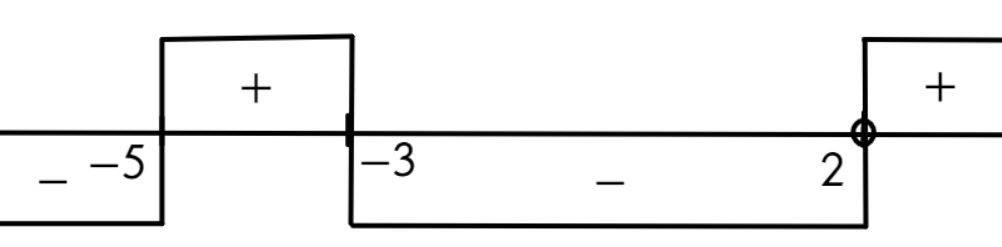
\includegraphics[scale=0.35]{isl69.png}}
\end{figure}
$x\in[-5;-3]\cup(2;+\infty).$\\
70. Необходимо выполнение двух условий: $\begin{cases} x^2-6x+8\geqslant0,\\ x-5\neq0.\end{cases}\Leftrightarrow
\begin{cases} (x-2)(x-4)\geqslant0,\\ x-5\neq0.\end{cases}
\Leftrightarrow$\\$ x\in (-\infty;2]\cup[4;5)\cup(5;+\infty).$\\
71. Необходимо выполнение двух условий: $\begin{cases} x^2-7x+12\geqslant0,\\ x-6\neq0.\end{cases}\Leftrightarrow
\begin{cases} (x-3)(x-4)\geqslant0,\\ x-6\neq0.\end{cases}
\Leftrightarrow$\\$ x\in (-\infty;3]\cup[4;6)\cup(6;+\infty).$\\
72. Уравнение имеет только положительные корни при выполнении следующих условий: эти корни существуют (то есть $D\geqslant0),$ их сумма и произведение положительны (эти условия мы будем проверять при помощи теоремы Виета). Запишем эти условия в виде системы неравенств и решим её: $\begin{cases} 4-4\cdot7\cdot4k\geqslant0,\\
\cfrac{2}{7}>0,\\ \cfrac{4k}{7}>0.\end{cases}\Leftrightarrow\begin{cases} k\leqslant\cfrac{1}{28},\\ k>0\end{cases}\Leftrightarrow
k\in \left(0;\cfrac{1}{28}\right].$\\
73. Уравнение имеет только положительные корни при выполнении следующих условий: эти корни существуют (то есть $D\geqslant0),$ их сумма и произведение положительны (эти условия мы будем проверять при помощи теоремы Виета). Запишем эти условия в виде системы неравенств и решим её: $\begin{cases} 4-4\cdot3\cdot9k\geqslant0,\\
\cfrac{2}{3}>0,\\ \cfrac{9k}{3}>0.\end{cases}\Leftrightarrow\begin{cases} k\leqslant\cfrac{1}{27},\\ k>0\end{cases}\Leftrightarrow
k\in \left(0;\cfrac{1}{27}\right].$\\
74. Выразим $y:\ y=3-\cfrac{3}{2}x.$ Если $x\in(-8;8),$ то $\cfrac{3}{2}x\in (-12;12),\ 3-\cfrac{3}{2}x\in (-9;15).$\\
75. Выразим $x:\ x=2-\cfrac{3}{4}y.$ Если $y\in(-12;12),$ то $\cfrac{3}{4}y\in (-9;9),\ 2-\cfrac{3}{4}y\in (-7;11).$\\
76. Для того, чтобы число 1 находилось между корнями уравнения, необходимо и достаточно выполнение двух условий. Во-первых, эти корней должно быть два, то есть $D>0.$ Во-вторых, выражение $(x_1-1)(x_2-1)$ должно быть отрицательно (это гарантирует, что скобки разных знаков, а значит один корень больше 1, а другой меньше). Запишем эти условия в виде системы неравенств и решим её, воспользовавшись теоремой Виета:\\
$\begin{cases}(a+1)^2+4a^2>0,\\ (x_1-1)(x_2-1)<0.\end{cases}\Leftrightarrow x_1x_2-(x_1+x_2)+1<0\Leftrightarrow
-a^2+a+1+1<0\Leftrightarrow a^2-a-2>0\Leftrightarrow (a-2)(a+1)>0\Leftrightarrow a\in (-\infty;-1)\cup(2;+\infty).$\\
77. Для того, чтобы число 1 находилось между корнями уравнения, необходимо и достаточно выполнение двух условий. Во-первых, эти корней должно быть два, то есть $D>0.$ Во-вторых, выражение $(x_1-1)(x_2-1)$ должно быть отрицательно (это гарантирует, что скобки разных знаков, а значит один корень больше 1, а другой меньше). Запишем эти условия в виде системы неравенств и решим её, воспользовавшись теоремой Виета:\\
$\begin{cases}(1-a)^2+4a^2>0,\\ (x_1-1)(x_2-1)<0.\end{cases}\Leftrightarrow x_1x_2-(x_1+x_2)+1<0\Leftrightarrow
-a^2+1-a+1<0\Leftrightarrow a^2+a-2>0\Leftrightarrow (a+2)(a-1)>0\Leftrightarrow a\in (-\infty;-2)\cup(1;+\infty).$\\
78. По теореме Виета $x_1+x_2=15,\ x_1x_2=q.$ Тогда $\cfrac{1}{x_1}+\cfrac{1}{x_2}=\cfrac{x_1+x_2}{x_1x_2}=\cfrac{15}{q}=\cfrac{5}{12}\Rightarrow q=36.$ Необходимо решить уравнение $x^2-15x+36=0,\ (x-3)(x-12)=0,\ x=3$ или $x=12.$\\
79. По теореме Виета $x_1+x_2=-p,\ x_1x_2=36.$ Тогда $\cfrac{1}{x_1}+\cfrac{1}{x_2}=\cfrac{x_1+x_2}{x_1x_2}=\cfrac{-p}{36}=\cfrac{5}{12}\Rightarrow p=-15.$ Необходимо решить уравнение $x^2-15x+36=0,\ (x-3)(x-12)=0,\ x=3$ или $x=12.$\\
80. Квадратное уравнение может иметь более 2 корней только если оно вырождается в уравнение $0=0,$ которое имеет бесконечно много корней. Свободный член $4a-4$ равен нулю только при $a=1,$ при этом же значении $a$ равны нулю и остальные коэффициенты. Поэтому $a=1$ является правильным ответом.\\
81. Квадратное уравнение может иметь более 2 корней только если оно вырождается в уравнение $0=0,$ которое имеет бесконечно много корней. Свободный член $-3a+3$ равен нулю только при $a=1,$ при этом же значении $a$ равны нулю и остальные коэффициенты. Поэтому $a=1$ является правильным ответом.\\
82. По теореме Виета $x_1+x_2=4,\ x_1x_2=-1.$ Тогда $x_1^3+x_2^3=(x_1+x_2)(x_1^2-x_1x_2+x_2^2)=(x_1+x_2)((x_1+x_2)^2-3x_1x_2)=4\cdot(16+3)=76.$\\
83. По теореме Виета $x_1+x_2=3,\ x_1x_2=-2.$ Тогда $x_1^3+x_2^3=(x_1+x_2)(x_1^2-x_1x_2+x_2^2)=(x_1+x_2)((x_1+x_2)^2-3x_1x_2)=3\cdot(9+6)=45.$\\
84. Подставим значение $3:\ 27-9+3b+24=0,\ 3b=-42,\ b=-14.$ Так как 3 является корнем многочлена $x^3-x^2-14x+24,$ по теореме Безу его можно поделить на $x-3.$ Можно сделать это столбиком или схемой Горнера, но здесь мы сделаем это при помощи выделения соответствующих множителей.
$x^3-x^2-14x+24=x^2(x-3)+2x(x-3)-8(x-3)=(x-3)(x^2+2x-8)=(x-3)(x+4)(x-2)=0.$ Таким образом, $x\in\{-4; 2; 3\}.$\\
85. Подставим значение $-2:\ -8+4-2b-24=0,\ 2b=-28,\ b=-14.$ Так как $-2$ является корнем многочлена $x^3+x^2-14x-24,$ по теореме Безу его можно поделить на $x+2.$ Можно сделать это столбиком или схемой Горнера, но здесь мы сделаем это при помощи выделения соответствующих множителей.
$x^3+x^2-14x-24=x^2(x+2)-x(x+2)-12(x+2)=(x+2)(x^2-x-12)=(x+2)(x-4)(x+3).$ Таким образом, $x\in\{-3; -2; 4\}.$\\
86. $6-2x^2-2xy-6x-y^2=-(2x^2+2xy+6x+y^2-6)=-(x^2+2xy+y^2+x^2+6x+9-15)=-(x+y)^2-(x+3)^2+15.$ Наибольшее значение принимается, когда квадраты равны 0, то есть $x+3=0,\ x=-3,\ x+y=0,\ y=-x=3.$\\
87. $20-2x^2+2xy-4x-y^2=-(2x^2-2xy+y^2+4x-20)=-(x^2-2xy+y^2+x^2+4x+4-24)=-(x-y)^2-(x+2)^2+24.$ Наибольшее значение принимается, когда квадраты равны 0, то есть $x+2=0,\ x=-2,\ x-y=0,\ y=x=-2.$\\
88. Возможны два случая: $D=0$ или $a=0.$ В первом случае $4(a-2)^2-4a(a+1)=0,\ a^2-4a+4-a^2-a=0,\ a=\cfrac{4}{5}.$ Во втором случае $a=0,\ x=-\cfrac{1}{4}.$\\
89. Возможны два случая: $D=0$ или $a=0.$ В первом случае $16(a-1)^2-4a(4a-3)=0,\ 4a^2-8a+4-4a^2+3a=0,\ a=\cfrac{4}{5}.$ Во втором случае $a=0,\ x=-\cfrac{3}{4}.$\newpage\noindent
90. По теореме Виета $x_1+x_2=a^2-5a=a(a-5)<0\Leftrightarrow a\in(0;5).$ Также необходимо проверить, что корни существуют, то есть $D\geqslant0,\ (a^2-5a)^2-4\cdot4a^2=(a^2-5a-4a)(a^2-5a+4a)=a(a-9)a(a-1)=a^2(a-9)(a-1)\geqslant0.$ Применив метод интервалов, найдём ответ:
\begin{figure}[ht!]
\center{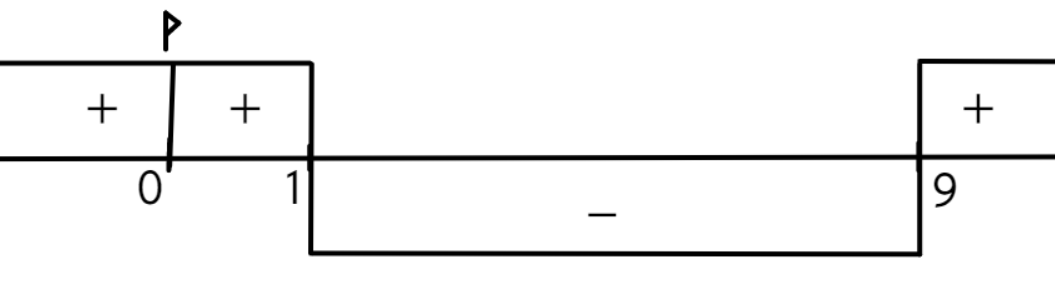
\includegraphics[scale=0.35]{isl90.png}}
\end{figure}
$a\in[-\infty;1]\cup[9;+\infty).$\\ Окончательным ответом в задаче будет пересечение полученных ответов, $a\in (0;1].$\\
91. По теореме Виета $x_1+x_2=5a-a^2=a(5-a)>0\Leftrightarrow a\in(0;5).$ Также необходимо проверить, что корни существуют, то есть $D\geqslant0,\ (a^2-5a)^2-4\cdot4a^2=(a^2-5a-4a)(a^2-5a+4a)=a(a-9)a(a-1)=a^2(a-9)(a-1)\geqslant0.$ Применив метод интервалов, найдём ответ:
\begin{figure}[ht!]
\center{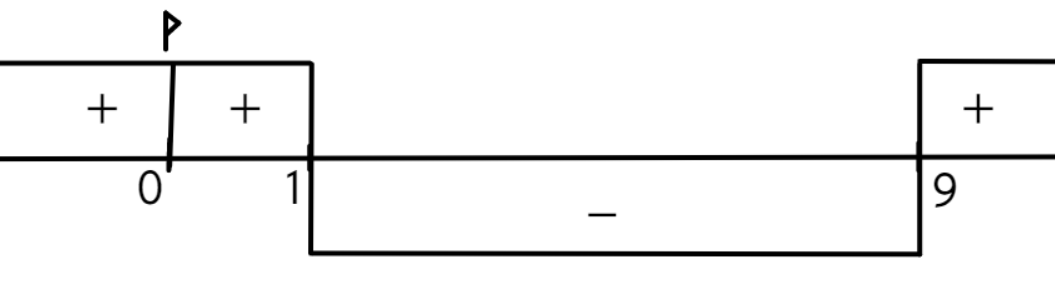
\includegraphics[scale=0.35]{isl90.png}}
\end{figure}
$a\in[-\infty;1]\cup[9;+\infty).$\\ Окончательным ответом в задаче будет пересечение полученных ответов, $a\in (0;1].$\\
92. $(x-5)(2x-a)=x-5\Leftrightarrow(x-5)(2x-a-1)=0\Leftrightarrow \left[\begin{array}{l}x=5,\\ x=\cfrac{a+1}{2}.\end{array}\right.$
Если корень ровно один, то $\cfrac{a+1}{2}=5,\ a=9.$\\
93. $(x-3)(2x-a)=x-3\Leftrightarrow(x-3)(2x-a-1)=0\Leftrightarrow \left[\begin{array}{l}x=3,\\ x=\cfrac{a+1}{2}.\end{array}\right.$
Если корень ровно один, то $\cfrac{a+1}{2}=3,\ a=5.$\\
94. $ax=|x-2|\Leftrightarrow \begin{cases}\left[\begin{array}{l}x-2=ax,\\ x-2=-ax.\end{array}\right.\\ ax\geqslant0.\end{cases}\Leftrightarrow
\begin{cases}\left[\begin{array}{l}x(1-a)=2,\\ x(1+a)=2.\end{array}\right.\\ ax\geqslant0.\end{cases}$
Так как $a>0,$ корень $x=\cfrac{2}{1+a}>0$ всегда подходит. Значит, не подходить должен корень $x=\cfrac{2}{1-a}.$ Это может произойти из-за нуля в знаменателе $(a=1)$ или из-за того, что он отрицателен, то есть $1-a<0,\ a>1.$ Таким образом, при положительных $a$ уравнение имеет единственное решение при $a\in[1;+\infty).$\\
95. Необходимо выполнение системы неравенств:\\ $\begin{cases} 24-x^2\geqslant0,\\ x^2+x-20>0.\end{cases}\Leftrightarrow
\begin{cases} (2\sqrt{6}-x)(2\sqrt{6}+x)\geqslant0,\\ (x-4)(x+5)>0.\end{cases}\Leftrightarrow
\begin{cases} x\in[-2\sqrt{6};2\sqrt{6}],\\ x\in(-\infty;-5)\cup(4;+\infty).\end{cases}\Leftrightarrow x\in(4;2\sqrt{6}].$\\
96. $ax=|x+2|\Leftrightarrow \begin{cases}\left[\begin{array}{l}x+2=ax,\\ x+2=-ax.\end{array}\right.\\ ax\geqslant0.\end{cases}\Leftrightarrow
\begin{cases}\left[\begin{array}{l}x(a-1)=2,\\ x(a+1)=-2.\end{array}\right.\\ ax\geqslant0.\end{cases}$
Во-первых, один корень у этого уравнения может быть из-за того, что при вычислении второго получается 0 в знаменателе, тогда $a=1$ или $a=-1.$ При $a=1$ имеем корень $x=-1,$ который не удовлетворяет условию $ax\geqslant0,$ а при $a=-1$ --- $x=-1$ этому условию удовлетворяет. Поэтому при $a=1$ корней нет вообще, а при $a=-1$ он как раз один. При положительных значениях $a$ корень $x=-\cfrac{2}{a+1}<0,$ а значит не подходит. Поэтому должен подходить второй корень, значит $a-1>0,\ a>1.$ При отрицательных значениях $a$ корень $x=\cfrac{2}{a-1}<0$ точно подходит, значит второй корень должен не подходить. Поэтому $a+1<0,\ a<-1.$ Также корни могут совпадать, $\cfrac{2}{a-1}=-\cfrac{2}{a+1},\ a-1=-a-1,\ a=0.$ Таким образом, один корень данное уравнение имеет при $a\in(-\infty;-1]\cup\{0\}\cup(1;+\infty).$\\
97. $\begin{cases}
(k+2)x+3y=9+kx,\\
x+(k+4)y=2.
\end{cases}\Leftrightarrow\begin{cases}
2x+3y=9,\\
x+(k+4)y=2.
\end{cases}\Leftrightarrow\begin{cases}
2x+3y=9,\\
(2k+5)y=-5.
\end{cases}$
У этой системы не может быть бесконечно много решений: из второго уравнения однозначно определяется $y,$ а потом из первого уравнения определяется $x.$ Если $2k+5\neq0,$ то у системы одно решение, а при $2k+5=0$ --- ни одного.\\
98. $(ax^2+3x+1)(x-3)=(x-3)\Leftrightarrow (x-3)(ax^2+3x+1-1)=0\Leftrightarrow (x-3)x(ax+3)=0.$ У этого уравнения при любом значении $a$ точно есть решения $x=3$ и $x=0,$ значит одного решения у него быть не может.\\
99. По теореме Виета $x_1+x_2=a^2-5a=a(a-5)<0\Rightarrow a\in(0;5).$ Также необходимо проверить существование корней, то есть $D=(a^2-5a)^2-16=
(a^2-5a-4)(a^2-5a+4)=$\\$\left(a-\cfrac{5-\sqrt{41}}{2}\right)\left(a-\cfrac{5+\sqrt{41}}{2}\right)(a-4)(a-1)\geqslant0.$\\ Применив метод интервалов, найдём ответ:
\begin{figure}[ht!]
\center{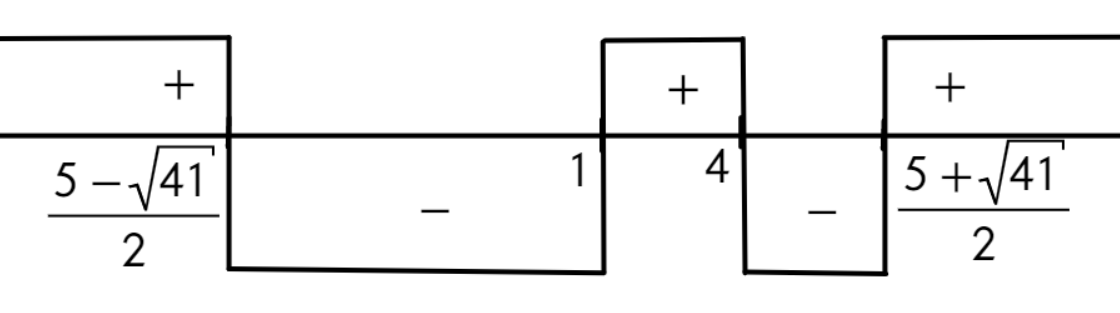
\includegraphics[scale=0.35]{isl99.png}}
\end{figure}
$a\in\left(-\infty;\cfrac{5-\sqrt{41}}{2}\right]\cup[1;4]\cup\left[\cfrac{5+\sqrt{41}}{2};+\infty\right).$
Окончательным ответом в задаче будет пересечение полученных ответов, $a\in [1;4].$\\
100. По теореме Виета $x_1+x_2=\cfrac{7}{2},\ x_1x_2=2.$ Тогда $\cfrac{x_1^2}{x_2}+\cfrac{x_2^2}{x_1}=\cfrac{x_1^3+x_2^3}{x_1x_2}=\cfrac{(x_1+x_2)(x_1^2-x_1x_2+x_2^2)}{x_1x_2}=
\cfrac{(x_1+x_2)((x_1+x_2)^2-3x_1x_2)}{x_1x_2}=\cfrac{\cfrac{7}{2}\cdot\left(\cfrac{49}{4}-6\right)}{2}=\cfrac{175}{16}.$\\
101. а) Подставим $x=3:\ 7\cdot9-2\cdot3+4a=0,\ a=-\cfrac{57}{4}.$\\
б) Для этого должно выполняться неравенство $D=4-4\cdot7\cdot4a>0,\ 28a<1,\ a\in\left(-\infty;\cfrac{1}{28}\right).$\\
в) Сумма корней по теореме Виета равна $\cfrac{2}{7}>0,$ также положительно должно быть их произведение $\cfrac{4a}{7}>0,\ a>0.$ При этом корень может быть и один, поэтому в отличие от пункта б) $a=\cfrac{1}{28}$ также подходит. Таким образом, ответ $a\in\left(0;\cfrac{1}{28}\right].$\\
г) При $a<0$ согласно пункту а) корни есть, при этом их произведение отрицательно, значит среди них точно есть отрицательный. При $a=0$ корни $x=0$ и $x=\cfrac{2}{7},$ отрицательных нет. При $a\in\left(0;\cfrac{1}{28}\right]$ согласно пункту в) оба корня положительны, а при $a>\cfrac{1}{28}$ корней нет вообще, а значит нет и отрицательных. Таким образом, ответ $a\in[0;+\infty).$\\
102. а) Два корня квадратное уравнение имеет при $D=a^2-4(a-1)=(a-2)^2>0,\ a\neq2.$\\
б) Уравнение $\cfrac{x^2-ax+a-1}{x+5}=0$ имеет единственное решение либо когда уравнение $x^2-ax+a-1=0$ имеет единственное решение, отличное от $-5,$ либо когда один из корней этого уравнения равен $-5.$ По пункту а) единственное решение при $a=2,$ тогда $x=1.$ Подставим $x=-5,$ имеем $25+5a+a-1=0,\ 6a=-24,\ a=-4.$ Таким образом, $a\in\{-4;2\}.$\\
103. а) Два корня квадратное уравнение имеет при $D=a^2-4(3a-9)=(a-6)^2>0,\ a\neq6.$\\
б) Уравнение $\cfrac{x^2-ax+3a-9}{x-4}=0$ имеет единственное решение либо когда уравнение $x^2-ax+3a-9=0$ имеет единственное решение, отличное от $4,$ либо когда один из корней этого уравнения равен $4.$ По пункту а) единственное решение при $a=6,$ тогда $x=3.$ Подставим $x=4,$ имеем $16-4a+3a-9=0,\ a=7.$ Таким образом, $a\in\{6;7\}.$\\
104. Возможны два случая: $D=0$ или $a-2=0.$ В первом случае $4(a-2)^2-4(a-2)\cdot3=0,\ (a-2)(a-5)=0, a=2$ или $a=5.$ Но при $a=2$ обнуляется ещё и старший коэффициент и получается уравнение $3=0,$ корней у которого нет вообще. Таким образом, подходит только $a=5.$\\
105. Возможны два случая: $D=0$ или $a+3=0.$ В первом случае $4(a+3)^2+4(a+3)\cdot5=0,\ (a+3)(a+8)=0, a=-3$ или $a=-8.$ Но при $a=-3$ обнуляется ещё и старший коэффициент и получается уравнение $-5=0,$ корней у которого нет вообще. Таким образом, подходит только $a=-8.$\\
106. Раз график не проходит через III четверть, он пересекает ось ординат выше нуля, поэтому $b>0.$ Также при больших по модулю отрицательных значениях $x$ значения $y$ должны быть положительны (так как график в II четверти, а не в III), поэтому $a<0.$\\
107. Раз график не проходит через II четверть, он пересекает ось ординат ниже нуля, поэтому $b<0.$ Также при больших по модулю отрицательных значениях $x$ значения $y$ должны быть отрицательны (так как график в III четверти, а не во II), поэтому $a>0.$\\
108. Раз решением является промежуток, $a<0,$ иначе подходили бы очень большие положительные значения $x.$ По теореме Виета $x_1x_2=\cfrac{c}{a}<0\Rightarrow c>0.$\\
109. Раз решением является промежуток, $a>0,$ иначе подходили бы очень большие положительные значения $x.$ По теореме Виета $x_1x_2=\cfrac{c}{a}<0\Rightarrow c<0.$\\
110. $\cfrac{10}{x^2+y^2+4x-6y+14}=\cfrac{10}{(x+2)^2+(y-3)^2+1}.$ Наибольшее значение дроби достигается, когда знаменатель достигает наименьшее значение, а это происходит, когда квадраты равны нулю. Значит, $x=-2,\ y=3,$ значение равно 10.\\
111. $\cfrac{8}{x^2+y^2-2x-10y+30}=\cfrac{8}{(x-1)^2+(y-5)^2+4}.$ Наибольшее значение дроби достигается, когда знаменатель достигает наименьшее значение, а это происходит, когда квадраты равны нулю. Значит, $x=1,\ y=5,$ значение равно 2.\\
112. Необходимо и достаточно, чтобы выполнялось неравенство $\cfrac{1-2x}{3x+5}+2\geqslant0\Leftrightarrow\cfrac{1-2x+6x+10}{3x+5}\geqslant0\Leftrightarrow
\cfrac{4x+11}{3x+5}\geqslant0\Leftrightarrow x\in\left(-\infty;-\cfrac{11}{4}\right]\cup\left(-\cfrac{5}{3};+\infty\right).$\\
113. Необходимо и достаточно, чтобы выполнялось неравенство $\cfrac{5+6x}{3x+4}-1\geqslant0\Leftrightarrow\cfrac{5+6x-3x-4}{3x+4}\geqslant0\Leftrightarrow
\cfrac{3x+1}{3x+4}\geqslant0\Leftrightarrow x\in\left(-\infty;-\cfrac{4}{3}\right)\cup\left[-\cfrac{1}{3};+\infty\right).$\\
114. По теореме Виета $x_1+x_2=3,\ x_1x_2=a.$ Тогда $(x_1-x_2)^2=(x_1+x_2)^2-4x_1x_2=9-4a=25,\ a=-4.$ При этом $D=9+16>0,$ значит корни существуют и $a=-4$ является ответом.\\
115. Выражение принимает наименьшее значение, когда оба подкоренных выражения равны нулю, то есть $\begin{cases} 2x+2y+10=0,\\ x+3y-3=0.\end{cases}
\Leftrightarrow \begin{cases} -4y+16=0,\\ x+3y-3=0.\end{cases}\Leftrightarrow \begin{cases} y=4,\\ x=-9.\end{cases}$ Итак, наименьшее значение равно 0 и достигается оно при $x=-9,\ y=4.$\\
116. Выражение принимает наименьшее значение, когда оба подкоренных выражения равны нулю, то есть $\begin{cases} 2x-2y+10=0,\\ x+3y-3=0.\end{cases}
\Leftrightarrow \begin{cases} -8y+16=0,\\ x+3y-3=0.\end{cases}\Leftrightarrow \begin{cases} y=2,\\ x=-3.\end{cases}$ Итак, наименьшее значение равно 0 и достигается оно при $x=-3,\ y=2.$\\
117. По теореме Виета $x_1+x_2=2,\ x_1x_2=-1,$ тогда $x_1^2+x_2^2=(x_1+x_2)^2-2x_1x_2=4+2=6.$\\
118. По теореме Виета $x_1+x_2=15,\ x_1x_2=q,$ тогда $x_1^2+x_2^2=(x_1+x_2)^2-2x_1x_2=225-2q=125,$ откуда $q=(225-125):2=50.$ Таким образом, необходимо решить уравнение $x^2-15x+50=0,\ (x-10)(x-5)=0,\ x=5$ или $x=10.$\\
119. По теореме Виета $x_1+x_2=5,\ x_1x_2=q,$ тогда $x_1^2+x_2^2=(x_1+x_2)^2-2x_1x_2=25-2q=125,$ откуда $q=(25-125):2=-50.$ Таким образом, необходимо решить уравнение $x^2-5x-50=0,\ (x-10)(x+5)=0,\ x=10$ или $x=-5.$\\
120. Выразим $y=6-x,$ тогда $xy=x(6-x)=6x-x^2=-(x^2-6x)=-((x-3)^2-9)=9-(x-3)^2\leqslant 9.$\\
121. Выразим $y=8-x,$ тогда $xy=x(8-x)=8x-x^2=-(x^2-8x)=-((x-4)^2-16)=16-(x-4)^2\leqslant 16.$\\
122. Квадратное уравнение имеет единственное решение либо если коэффициент при $x^2$ равен нулю, либо если равен нулю дискриминант. В первом случае $a=0,$ во втором случае $\cfrac{D}{4}=(1-a)^2+4a=1-2a+a^2+4a=a^2+2a+1=(a+1)^2=0,\ a=-1.$\\
123. Квадратное уравнение имеет единственное решение либо если коэффициент при $x^2$ равен нулю, либо если равен нулю дискриминант. В первом случае $a=0,$ во втором случае $\cfrac{D}{4}=(1+a)^2-4a=1+2a+a^2-4a=a^2-2a+1=(a-1)^2=0,\ a=1.$\\
124. $\cfrac{(x-a)(x-2a)}{x-3a}=0\Leftrightarrow \begin{cases} \left[\begin{array}{l} x=a,\\ x=2a.\end{array}\right.\\ x\neq 3a.\end{cases}$ Уравнение не имеет решений, если оба его возможных корня совпадают с запрещённым значением, то есть $a=2a=3a,$ откуда $a=0.$\\
125. $\cfrac{(x-a)(x-4a)}{x-2a}=0\Leftrightarrow \begin{cases} \left[\begin{array}{l} x=a,\\ x=4a.\end{array}\right.\\ x\neq 2a.\end{cases}$ Уравнение не имеет решений, если оба его возможных корня совпадают с запрещённым значением, то есть $a=4a=2a,$ откуда $a=0.$\\
126. $2|x-1|\geqslant a-x\Leftrightarrow a\leqslant  2|x-1|+x.$ Это неравенство выполнено при всех значениях $x$ тогда, когда значение параметра $a$ не превосходит минимального значения правой части. $f(x)=2|x-1|+x=\left[\begin{array}{l}\begin{cases}2x-2+x,\\ x\geqslant 1. \end{cases}\\ \begin{cases}-2x+2+x,\\ x< 1. \end{cases}\end{array}\right.\Leftrightarrow\left[\begin{array}{l}\begin{cases}3x-2,\\ x\geqslant 1. \end{cases}\\ \begin{cases}2-x,\\ x<1. \end{cases}\end{array}\right.$ Минимальное значение $f(x)$ равно 1, значит $a\leqslant1.$\\
127. $2|x+1|\geqslant x-a\Leftrightarrow a\geqslant  x-2|x+1|.$ Это неравенство выполнено при всех значениях $x$ тогда, когда значение параметра $a$ не меньше максимального значения правой части. $f(x)=x-2|x+1|=\left[\begin{array}{l}\begin{cases}x-2x-2,\\ x\geqslant -1. \end{cases}\\ \begin{cases}x+2x+2,\\ x< -1. \end{cases}\end{array}\right.\Leftrightarrow\left[\begin{array}{l}\begin{cases}-x-2,\\ x\geqslant -1. \end{cases}\\ \begin{cases}3x+2,\\ x<-1. \end{cases}\end{array}\right.$ Максимальное значение $f(x)$ равно $-1,$ значит $a\geqslant-1.$\\
128. Минимальное значение модуля равно 0 при $a=1,\ b=2.$ Максимальное значение модуля равно 9 при $a=-2,\ b=5.$\\
129. Минимальное значение модуля равно 0 при $a=1,\ b=2.$ Максимальное значение модуля равно 9 при $a=-2,\ b=5.$\\
130. Выразим $x=y+2,$ тогда $x^2+y^2=y^2+4y+4+y^2=2y^2+4y+4=2(y^2+2y+2)=2((y+1)^2+1)\geqslant2.$\\
131. Выразим $x=y-2,$ тогда $x^2+y^2=y^2-4y+4+y^2=2y^2-4y+4=2(y^2-2y+2)=2((y-1)^2+1)\geqslant2.$\\
132. Составим уравнение для нахождения точки пересечения: $kx-k=-x^2,\ x^2+kx-k=0.$ Парабола и прямая не имеют общих точек, если у этого уравнения нет корней, то есть если $D<0,$\\ $k^2+4k<0,\ k(k+4)<0,\ k\in(-4;0).$\\
133. У этого уравнения может быть только один корень в двух случаях. Во-первых, у числителя может быть один корень, не равный 2. Для этого уравнение $(2p-3)x^2-(3p+2)x+p-1=0$ должно быть линейным или его дискриминант должен быть равен нулю. Уравнение линейно при $2p-3=0,\ p=\cfrac{3}{2},$ тогда $\cfrac{13}{2}x+\cfrac{1}{2}=0,\ x=-13,$ это значение $p$ подходит. Дискриминант равен нулю при $(3p+2)^2-4(2p-3)(p-1)=0,\ p^2+32p-8=0,\ p=-16\pm2\sqrt{66}.$ При этих значениях $p$ единственный корень также не равен 2. Во втором случае, подставив 2 в числитель и приравняв его к нулю, получим $8p-12-6p-4+p-1=0,\ 3p-17=0,\ p=\cfrac{17}{3}.$ Все найденные значения $p$ подходят, таким образом $p\in\left\{-16\pm2\sqrt{66};\cfrac{3}{2};\cfrac{17}{3}\right\}.$\\
134. У этого уравнения может быть только один корень в двух случаях. Во-первых, у числителя может быть один корень, не равный $-3.$ Для этого уравнение $(2q+1)x^2+(3q-2)x+q+2=0$ должно быть линейным или его дискриминант должен быть равен нулю. Уравнение линейно при $2q+1=0,\ q=-\cfrac{1}{2},$ тогда $-\cfrac{7}{2}x+\cfrac{3}{2}=0,\ x=\cfrac{3}{7},$ это значение $q$ подходит. Дискриминант равен нулю при $(3q-2)^2-4(2q+1)(q+2)=0,\ q^2-32q-4=0,\ q=16\pm2\sqrt{65}.$ При этих значениях $q$ единственный корень также не равен $-3.$ Во втором случае, подставив $-3$ в числитель и приравняв его к нулю, получим $18q+9-9q+6+q+2=0,\ 10q+17=0,\ q=-\cfrac{17}{10}.$ Все найденные значения $q$ подходят, таким образом $p\in\left\{16\pm2\sqrt{65};-\cfrac{1}{2};-\cfrac{17}{10}\right\}.$\\
135. По теореме Виета имеем соотношения $x_1+x_2=-\cfrac{2}{3},\ x_1x_2=-3.$ Пусть $y_1=\cfrac{2-x_1}{x_2},\ y_2=\cfrac{2-x_2}{x_1},$ тогда выполняются равенства
$y_1+y_2=\cfrac{2-x_1}{x_2}+\cfrac{2-x_2}{x_1}=\cfrac{2x_1-x_1^2+2x_2-x_2^2}{x_1x_2}=$\\$
\cfrac{2(x_1+x_2)-((x_2+x_2)^2-2x_1x_2)}{x_1x_2}=\cfrac{-\cfrac{4}{3}-\left(\cfrac{4}{9}+6\right)}{-3}=\cfrac{70}{27},\
y_1y_2=\cfrac{(2-x_1)(2-x_2)}{x_1x_2}=$\\$\cfrac{4-2(x_1+x_2)+x_1x_2}{x_1x_2}=\cfrac{4+\cfrac{4}{3}-3}{-3}=-\cfrac{7}{9}=-\cfrac{21}{27}.$ По обратной теореме Виета числа $y_1$ и $y_2$ являются корнями квадратного уравнения $27x^2-70x-21=0.$\\
136. По теореме Виета имеем соотношения $x_1+x_2=\cfrac{3}{2},\ x_1x_2=-4.$ Пусть $y_1=\cfrac{x_1-1}{x_2},\ y_2=\cfrac{x_2-1}{x_1},$ тогда выполняются равенства
$y_1+y_2=\cfrac{x_1-1}{x_2}+\cfrac{x_2-1}{x_1}=\cfrac{x_1^2-x_1+x_2^2-x_2}{x_1x_2}=$\\$\cfrac{(x_1+x_2)^2-2x_1x_2-(x_1+x_2)}{x_1x_2}=
\cfrac{\cfrac{9}{4}+8-\cfrac{3}{2}}{-4}=-\cfrac{35}{16},\ y_1y_2=\cfrac{(x_1-1)(x_2-1)}{x_1x_2}=\cfrac{x_1x_2-(x_1+x_2)+1}{x_1x_2}=
\cfrac{-4-\cfrac{3}{2}+1}{-4}=\cfrac{9}{8}=\cfrac{18}{16}.$ По обратной теореме Виета числа $y_1$ и $y_2$ являются корнями квадратного уравнения $16x^2+35x+18=0.$\\
137. Пусть $x=2t,\ y=t,\ z=3t,$ тогда $\cfrac{3x+2y+z}{2x-3y+z}=\cfrac{6t+2t+3t}{4t-3t+3t}=\cfrac{11t}{4t}=\cfrac{11}{4}.$\\
138. Пусть $x=3t, y=t,\ z=2t,$ тогда $\cfrac{2y-4x+z}{5x-3y+8z}=\cfrac{2t-12t+2t}{15t-3t+16t}=\cfrac{-8t}{28t}=-\cfrac{2}{7}.$\\
139. По теореме Виета имеем соотношения $x_1+x_2=-\cfrac{8}{3},\ x_1x_2=-\cfrac{1}{3},$ тогда $x_1x_2^3+x_2x_1^3=x_1x_2(x_1^2+x_2^2)=
x_1x_2((x_1+x_2)^2-2x_1x_2)=-\cfrac{1}{3}\cdot\left(\cfrac{64}{9}+\cfrac{2}{3}\right)=-\cfrac{70}{27}.$\\
140. По теореме Виета имеем соотношения $x_1+x_2=\cfrac{7}{2},\ x_1x_2=-\cfrac{3}{2},$ тогда $x_1x_2^3+x_2x_1^3=x_1x_2(x_1^2+x_2^2)=
x_1x_2((x_1+x_2)^2-2x_1x_2)=-\cfrac{3}{2}\cdot\left(\cfrac{49}{4}+3\right)=-\cfrac{183}{8}.$\\
141. Уравнение может иметь либо если оно становится линейным, либо если его дискриминант равен нулю. В первом случае $a=0,$ а во втором
$(a+3)^2+4a=0,\ a^2+6a+9+4a=0,\ a^2+10a+9=0,\ (a+1)(a+9)=0,\ a=-9$ или $a=-1.$\\
142. По теореме Виета имеем соотношения $x_1+x_2=\cfrac{3}{5},\ x_1x_2=-\cfrac{11}{5},$ откуда $x_1^3x_2+x_2^3x_1=x_1x_2(x_1^2+x_2^2)=
x_1x_2((x_1+x_2)^2-2x_1x_2)=-\cfrac{11}{5}\cdot\left(\cfrac{9}{25}+\cfrac{22}{5}\right)=
-\cfrac{1309}{125}.$\\
143. По теореме Виета имеем соотношения $x_1+x_2=-\cfrac{3}{5},\ x_1x_2=-\cfrac{13}{5},$ откуда $x_1^3x_2+x_2^3x_1=x_1x_2(x_1^2+x_2^2)=
x_1x_2((x_1+x_2)^2-2x_1x_2)=-\cfrac{13}{5}\cdot\left(\cfrac{9}{25}+\cfrac{26}{5}\right)=
-\cfrac{1807}{125}.$\\
144. $\cfrac{ax^2-(3a+2)x+8}{x^2-x-2}=0\Leftrightarrow \begin{cases}
ax^2-(3a+2)x+8=0,\\ (x-2)(x+1)\neq0.\end{cases}\Leftrightarrow \begin{cases}
ax^2-(3a+2)x+8=0,\\ x\notin\{-1;2\}.\end{cases}$ У этого уравнения может быть один корень либо если у квадратного уравнения он один и не совпадает с числами $-1$ и 2, либо если у квадратного уравнения два корня, но один из них совпадает с числом $-1$ или 2. В первом случае равен нулю может быть либо коэффициент при $x^2,$ либо дискриминант. Если $a=0,$ то $-2x+8=0,\ x=4,$ этот случай подходит. Если $(3a+2)^2-4\cdot a\cdot8=0,\ 9a^2+12a+4-32a=0,\
9a^2-20a+4=0,\ a=2$ или $a=\cfrac{2}{9}.$ Если $a=2,$ то $x=\cfrac{3\cdot2+2}{2\cdot2}=2,$ а значит у этого уравнения нет корней вообще. Если $a=\cfrac{2}{9},$ то $x=\cfrac{3\cdot\cfrac{2}{9}+2}{2\cdot\cfrac{2}{9}}=6,$ значит этот случай подходит. Случай, когда один из корней совпал с числом 2, мы уже разобрали. Если один из корней совпал с числом $-1,$ то $a+3a+2+8=0,\ 4a=-10,\ a=-\cfrac{5}{2},$ этот случай также подходит.\\
145. $\cfrac{ax^2-(5a+2)x+18}{x^2-x-6}=0\Leftrightarrow \begin{cases}
ax^2-(5a+2)x+18=0,\\ (x-3)(x+2)\neq0.\end{cases}\Leftrightarrow \begin{cases}
ax^2-(5a+2)x+18=0,\\ x\notin\{-2;3\}.\end{cases}$ У этого уравнения может быть один корень либо если у квадратного уравнения он один и не совпадает с числами $-2$ и 3, либо если у квадратного уравнения два корня, но один из них совпадает с числом $-2$ или 3. В первом случае равен нулю может быть либо коэффициент при $x^2,$ либо дискриминант. Если $a=0,$ то $-2x+18=0,\ x=9,$ этот случай подходит. Если $(5a+2)^2-4\cdot a\cdot18=0,\ 25a^2+20a+4-72a=0,\
25a^2-52a+4=0,\ a=2$ или $a=\cfrac{2}{25}.$ Если $a=2,$ то $x=\cfrac{5\cdot2+2}{2\cdot2}=3,$ а значит у этого уравнения нет корней вообще. Если $a=\cfrac{2}{25},$ то $x=\cfrac{5\cdot\cfrac{2}{25}+2}{2\cdot\cfrac{2}{25}}=15,$ значит этот случай подходит. Случай, когда один из корней совпал с числом 3, мы уже разобрали. Если один из корней совпал с числом $-2,$ то $4a+10a+4+18=0,\ 14a=-22,\ a=-\cfrac{11}{7},$ этот случай также подходит.\\
146. По теореме Виета $x_1x_2=a+3=-2,\ a=-5.$ При этом значении параметра $a$ уравнение имеет вид $x^2-10x-2=0,$ его дискриминант равен $100+8=108>0,$ значит такое $a$ существует.\\
147. По теореме Виета $x_1x_2=a+3=2,\ a=-1.$ При этом значении параметра $a$ уравнение имеет вид $x^2-2x+2=0,$ его дискриминант равен $4-8=-4<0,$ значит такого значения $a$ не существует.
\newpage
